\section{Model for Cloud Platforms}
\label{sec:modelcloud}
We will now consider the usage of model based methods for SQL-on-Hadoop engines on cloud platforms. Cloud based platforms have their own peculiarities that necessiates revisiting the algorithm proposed in the previous section. 

\subsection{Characteristics of Cloud platforms}
Cloud platforms provide additional flexibility due to the elastic nature of the cloud and the choice of different instance types.

\noindent\subsubsection*{Cloud elasticity}
 In the cloud, the physical resource for the cluster are not committed forever. Clusters can be spun up and shut down on demand. In the iterative and model based experiments till now, we have focused on the cumulative resource usage metric (Equation~\ref{eqn:totalresource}), which was mainly achieved by reducing the memory usage of the containers. 
In practice, this saving in memory would be useful only if it could be gainfully used by some other task or job. However, for all the big data SQL engines, the memory used by all the task processes is the same. It is controlled by parameters at the query level (e.g. mapper memory, reducer memory, spark executor memory)and cannot be tuned per task.
Further, each workload will use its own dynamic cluster in a Cloud setting, which implies that other workloads cannot use the memory saved either. 

Thus saving memory may not be very useful and should not be the main criterion. Let us look at memory allocation in further detail. In SQL-on-Hadoop systems, containers are allocated using Yarn, which allocates based on two dimensions - \textbf{memory} and \textbf{vcpu}. Each container is given 1 vcpu and some memory. If all the vcpus on a node are allocated and memory is still available, the extra memory cannot be used and is wasted. Conversely, if all memory is used up and extra vcpus are available, those extra vcpus are wasted since they cannot be allocated. 
Figure \ref{fig:container_shape} illustrates the three scenarios:
\begin{enumerate}[label=(\alph*)]
	\item[$\bullet$] Memory/vCPU ratio of container is same as that of instance; hence, neither memory nor CPU is wasted. 
	\item[$\bullet$] Memory/vCPU ratio of container is smaller than that of instance; hence, memory is wasted as extra memory of instance is still remaining unused after container allocation.
	\item[$\bullet$] Memory/vCPU ratio of container is higher than that of instance; hence, CPU is wasted as extra CPU of instance is remaining unused after container allocation.
\end{enumerate}
\begin{figure*}[h]
	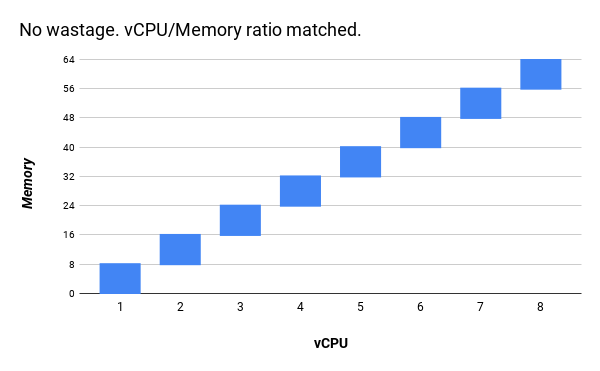
\includegraphics[width=0.3\linewidth]{container_shape1.png} 
	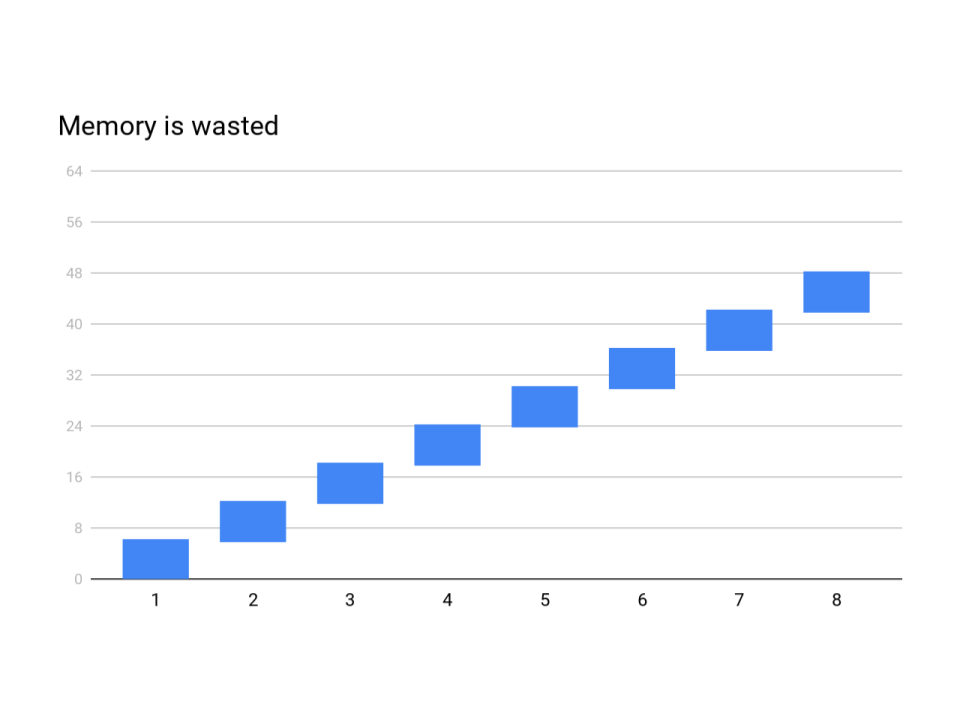
\includegraphics[width=0.3\linewidth]{container_shape2.png}
	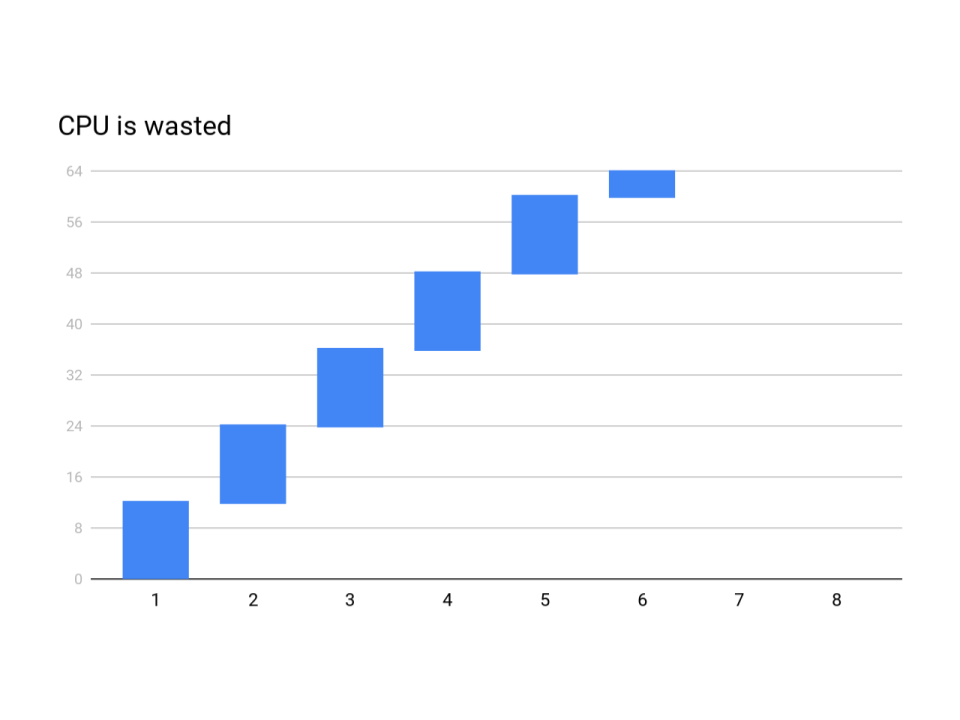
\includegraphics[width=0.3\linewidth]{container_shape3.png}
	%\vspace*{-15pt}
	\caption{\textbf{(a)} No Resource is wasted \textbf{(b)} Memory is wasted \textbf{(c)} CPU is wasted}
	\label{fig:container_shape}
\end{figure*}

This implies that memory for each container should be set according of the Memory/vCPU ratio of the machine which leads to the following conclusion:
\begin{insight}
	\label{insight:memcpu}
	For optimal usage of both memory and vcpus, the memory/vcpu ratio of the containers should match the memory/vcpu ratio of the machine type.
\end{insight}
Thus, the memory configuration parameter (mapper memory, reducer memory or spark executor memory) need not be optimized per query and is based on the machine characteristics. Further, since memory per container is fixed, the target metric to be optimized should be the cumulative cpu time (Equation~\ref{eqn:totaltime}) of the query rather than the resource utilization. 

\noindent\subsubsection*{Instance types}

Cloud platforms provide a choice of different instance types, each of which may have different dollar costs. Thus, it is important to recommend instance types along with configuration parameters. The metric that matters the most in this case is the total dollar cost (Equation~\ref{eqn:totalcost}).

\subsection{Algorithm}

\begin{algorithm}
	\caption{\textbf{fitJobMR}}\label{jobfit}
	\begin{algorithmic}[1]
		\footnotesize
		\REQUIRE  $\mathcal{M}$ is the job metrics (defined in table \ref{table:job_metrics} ), $I_{old}$  is instance configuration (defined in Table \ref{table:inst_conf}) on which $\mathcal{M}$ is collected, $I_{new}$ is new instance configuration on which $\mathcal{M}$ needs to be optimized upon, $\mathcal{G}$ is the global parameters defined in Table \ref{table:global_params}
		\ENSURE New Job parameter $\mathcal{P}_{new}$ (defined in table \ref{table:job_params}) that optimize the cumulative time of containers and predicted cumulative time of containers $\mathcal{T}$.
		\STATE newMemPerCore $\gets I_{new}$[nodeMemory] $/ I_{new}$[vCpuPerNode]
		\STATE $\mathcal{P}_{new}$[mapreduce.map.memory.mb] $\gets$ newMemPerCore
		\STATE $\mathcal{P}_{new}$[mapreduce.map.reduce.mb] $\gets$ newMemPerCore
		\STATE ioSort $\gets$ newMemPerCore $\times$ ioSortFrac
		\IF {ioSort $>$ $\mathcal{G}$[maxIOSort]}
		\STATE ioSort $\gets$ $\mathcal{G}$[maxIOSort]
		\ENDIF
		\STATE $\mathcal{P}_{new}$[mapreduce.task.io.sort.mb] $\gets$ ioSort
		\STATE outPerMap $\gets$ $\mathcal{M}$[mapperOutputBytes] $/$ $\mathcal{M}$[numOfMapper]
		\STATE newSplitSize $\gets$ $\mathcal{M}$[splitSize] $\times$ ioSort $/$ outPerMap
		\STATE $\mathcal{P}_{new}$[splitSize] $\gets$ newSplitSize
		\STATE newBPR $\gets$ ($\mathcal{M}$[reducerMemory] $\times$ $\mathcal{M}$[mapperInputBytes]) $/$ ($\mathcal{M}$[mapperOutputBytes] $\times$ $\mathcal{G}$[reducerFrac])  
		\STATE $\mathcal{P}_{new}$[hive.exec.reducers.bytes.per.reducer] $\gets$ newBPR
		\STATE predictedMapperTime $\gets$ $\mathcal{M}$[mapperTime] $\times$ ($\mathcal{M}$[mapperInputBytes] $/$ ($\mathcal{M}$[mapperInputBytes] + $\mathcal{M}$[spilledMapBytes])) $\times$ ($I_{old}$ [eCPU] $/$ $I_{new}$[eCPU])
		\STATE predictedReducerTime $\gets$ $\mathcal{M}$[reducerTime] $\times$ ($\mathcal{M}$[mapperOutputBytes] $/$ ($\mathcal{M}$[mapperOutputBytes] + $\mathcal{M}$[spilledRedBytes])) $\times$ ($I_{old}$ [eCPU] $/$ $I_{new}$[eCPU])
		\STATE $\mathcal{T}$ $\gets$ predictedMapperTime + predictedReducerTime
		\STATE \RETURN $\mathcal{P}_{new}$, $\mathcal{T}$
	\end{algorithmic}
\end{algorithm}

The algorithm consists of two parts -- \textbf{fitJobMR} (Algorithm\ref{jobfit}) that finds the optimal parameters on a given instance type for MR Job and $optimizeCost$ (Algorithm~\ref{cost_optimize}) that searches across instance types to determine the best instance type to be used. 

Algorithm \textbf{fitJobMR} is analogous to $OptResource$, but also takes the instance type $I_{new}$ as input. Instead of choosing the smallest possible $splitSize$ like $OptResource$, it starts with fixing $mapperMemory$ and $reducerMemory$ based on the memory available per core in the instance type being considered (lines 2--3). Based on this, the $ioSort$ is computed (lines 4--8). This is followed by computing the $splitSize$, such that the output of that split partition fits in the $ioSort$ and does not cause any spill (lines 9--11). Similarly, the $bytesPerReducer$ is computed such that the amount of mapper output data processed by each reducer fits in the reducer buffer without causing spills (lines 12--13). The algorithm also computes the estimated cumulative time.

Algorithm $optimizeCost$ searches for the best instance type. It iterates over all the available instance types and calls \textbf{fitJobMR} to find the best configuration and cumulative time for each type (line 2). It computes the dollar cost  of the query using the rental rate per core per unit time $r$ using Equation~\ref{eqn:totalcost} (line 3). The instance type leading to the least dollar cost and the configuration corresponding to that instance are finally output by the algorithm.

Algorithm \textbf{fitJobSpark} defined in Algorithm \ref{jobfitspark} is similar to \textbf{fitJobMR} but for SparkSQL Jobs instead of Hive on MR jobs. Algorithm \textbf{fitJobSpark} takes a set of stage parameters (defined in Table~\ref{table:stage_params}) $\mathcal{S}$ as input along with instance and global parameter as in \textbf{fitJobMR}.

\begin{table}[h]
\begin{tabular}{ |l|p {4.5 cm}| }
 \hline
 Parameters & Description \\ 
 \hline
 inputBytes  & Total Input Bytes Read \\ 
 shuffleRead & Shuffle Bytes Read\\ 
 \hline
\end{tabular}
\caption{Stage Parameter for SparkSQL Job}
\label{table:stage_params}
\end{table}

\renewcommand{\algorithmicrequire}{\textbf{Input:}}
\renewcommand{\algorithmicensure}{\textbf{Output:}}
\renewcommand{\algorithmiccomment}[1]{// #1}
\begin{algorithm}
\caption{\textbf{fitJobSpark}}\label{jobfitspark}
\begin{algorithmic}[1]
\footnotesize
\REQUIRE  $\mathcal{S}$ is set of stage parameters (defined in table \ref{table:stage_params} ), $\mathcal{I}$ is new instance configuration on which Spark Job needs to be optimized upon, $\mathcal{G}$ is the global parameters defined in Table \ref{table:global_params}, $\mathcal{T}$ is cumulative task time to execute job.
\ENSURE New Job parameter $\mathcal{P}_{new}$ (defined in table \ref{table:job_params}) that optimize the cumulative time of containers and predicted cumulative time of containers $\mathcal{T}_{new}$.
\STATE $\mathcal{P}_{new}$[spark.executor.cores] $\gets$ $\mathcal{I}$ [vCpuPerNode]
\STATE $\mathcal{P}_{new}$[spark.executor.memory] $\gets$ $\mathcal{I}$[nodeMemory] $\times$ $\mathcal{G}$[nodeMemoryFrac]
\STATE newMemPerCore $\gets$ ($\mathcal{I}$[nodeMemory] $\times$ $\mathcal{G}$[nodeMemoryFrac]) $/$ $\mathcal{I}$[vCpuPerNode]
\STATE shuffleBuffer $\gets$ newMemPerCore $\times$ $\mathcal{G}$[shuffleBufferFrac]
\STATE readBuffer $\gets$ newMemPerCore $\times$ $\mathcal{G}$[readBufferFrac]
\FOR {\textbf{each} $s_{i}$ $\in$ $\mathcal{S}$}
\STATE splitSize $\gets$ $min($ $s_{i}$[inputBytes] $/$  readBuffer, splitSize$)$ 
\STATE shufflePartiton $\gets$ $max($shuffleRead $/$ shuffleBuffer, shufflePartition$)$
\ENDFOR
\STATE $\mathcal{P}_{new}$[mapreduce.input.fileinputformat.split.maxsize] $\gets$ splitSize
\STATE $\mathcal{P}_{new}$[mapreduce.input.fileinputformat.split.minsize] $\gets$ splitSize
\STATE $\mathcal{P}_{new}$[spark.sql.shuffle.partition] $\gets$ shufflePartition
\STATE $\mathcal{T}_{new}$ $\gets$ $\mathcal{T}$ $\times$ ($I_{old}$ [eCPU] $/$ $I_{new}$[eCPU])
\RETURN $\mathcal{P}_{new}$, $\mathcal{T}_{new}$
\end{algorithmic}
\end{algorithm}

\begin{algorithm}
\caption{optimizeCost} \label{cost_optimize}
\begin{algorithmic}[1]
\footnotesize
\REQUIRE $\mathcal{P}$ is the job parameters (defined in \ref{table:job_params} ), Set $\mathcal{I} = {i_1, i_2, i_3, \ldots i_n} $ set of instance configurations (defined in \ref{table:inst_conf}), rental rates per core per unit time for each type $\mathcal{R}={r_1, r_2, \ldots r_n}$
\ENSURE Returns optimized instance type and job parameters across all the instance configurations in $\mathcal{I}$.
\FOR {$x$ = 1, 2 \ldots n}
	\STATE $config, time \gets fitJobForMR(\mathcal{P}, i_x)$
	\STATE $cost \gets  bestTime \times r_x$  
	\IF {$cost < bestCost$}
		\STATE $bestCost \gets cost$;
		$bestInstance \gets i_x$;
		$bestConfig \gets config$
	\ENDIF
\ENDFOR

\RETURN $bestInstance, bestConfig$
\end{algorithmic}
\end{algorithm}

\subsection{Results}

We evaluated the new cost metric defined for cloud on a synthetic workload as well as the same SparkSQL customer queries which were evaluated in Figure ~\ref{fig:modelbasedresultspark}. 

\subsubsection*{Synthetic Workload}
For the synthetic workload, we used the TPC DS dataset (scale 1000) and a subset of the queries. The experiments
were run on a 4-node cluster on AWS with machine type r3.4xlarge running SparkSQL on an Apache Spark cluster. We chose this specific machine type as it is the 
most popular machine type in Qubole Data Service. The cloud model suggested that it is cheaper to run these 
queries on c3 family of machines. We reran the queries on a 4-node cluster with machine type c3.4xlarge. 
Figure \ref{fig:syntheticcloudmodel} shows the reduction percent on absolute dollar cost of running a subset of the
TPC DS queries. Dollar cost is determined by the cost of running a particular AWS instance for cumulative time of running query as defined in Section~\ref{sec:optmethod}.
\begin{figure}[h]
	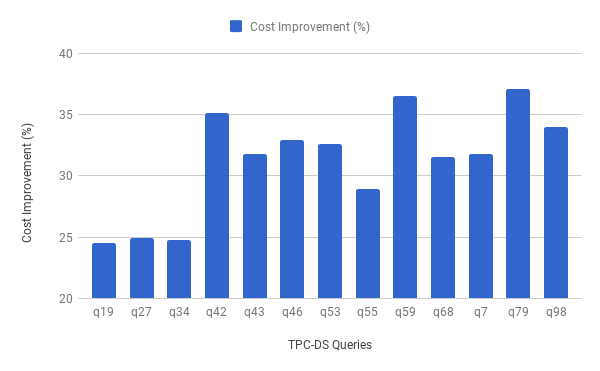
\includegraphics[width=\linewidth]{CloudSyn.png}
	%\vspace*{-15pt}
	\caption{Synthetic workload reduction in absolute dollar cost}
	\label{fig:syntheticcloudmodel}
\end{figure}

\subsubsection*{Real Workloads}
We ran our experiments on Amazon Web Services. Figure \ref{fig:modelbaseddollarresult} shows the reduction percent on absolute dollar cost of running 3 customer queries. 

\begin{figure}[h]
	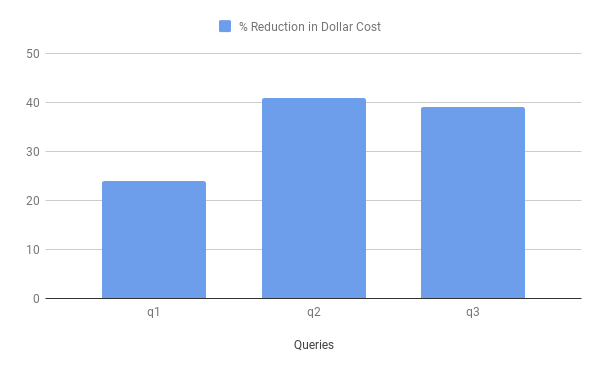
\includegraphics[width=\linewidth]{ModelExp.png}
	%\vspace*{-15pt}
	\caption{Real workload reduction in absolute dollar cost}
	\label{fig:modelbaseddollarresult}
\end{figure}
